\thispagestyle{fancy}
\chapter{Introduction} \label{ch:introduction}
\section*{\centering Chapter \thechapter}
\section*{\centering Introduction}

In the past few years, COVID-19 (Coronavirus Disease 2019) has rapidly become a pandemic. This disease, caused by a strain of the Corona virus, was discovered near the end of 2019, hence it was named COVID-19 disease. This disease primarily attacks the human respiratory system. The infected respiratory system leads to various complicated respiratory problems such as lung damage, pnuemonia, etc. The first reported case of COVID-19 was discovered in Wuhan, China. The disease spread in Wuhan rapidly, and after that, the disease began to spread world wide at an alarming rate. The World Health Organization soon classified the disease as a pandemic.

The infection of COVID-19 in patients showed extreme variation in severity. In some cases, the patients showed extremely mild symptoms, while in other cases, they developed extremely severe infections. The infection severity was heavily impacted by the comorbidities of patients. Patients with comorbidities result in server infections as well as lead to fatal cases. Paitents with prior comorbidities such as diabetes, cardiovascular diseases, and respiratory problems showed higher severity.

Cardiovascular comorbidities include various circulation disorders such as arrhythmia, artery diseases, hypertension, and heart diseases. Arrhythmia itself is a disorder, but it also serves as a symptom in other disorders. An arrhythmia is an irregular beating of the heart. This leads to either a faster heartbeat (tachycardia), a slower heartbeat (bradycardia), or a random beating pattern. Detection of arrhythmia suggest the possibility of other cardiovascular disorders, hence it is primary test in patients admitted due to COVID-19 infections.

The electrocardiogram signals, or ECG signals for short, are used to prepare charts. These charts are used to detect arrhythmia in patients. These ECG charts are recordings of human heartbeats. The ECG is generally taken with an 8-lead or 12-lead system. \Cref{fig:normal_abnormal_ecg_signal} shows the normal and abnormal ECG singals recorded on 12-leads. The heart rhythm is captured at a 120 Hz frequency. The chart is observed by a primary care physician. If the chart shows abnormalities, the patient is said to have arrhythmia. The patients with arrhythmias are further tested for other cardiovascular diseases or disorders.

\begin{figure}[ht]
  \centering
  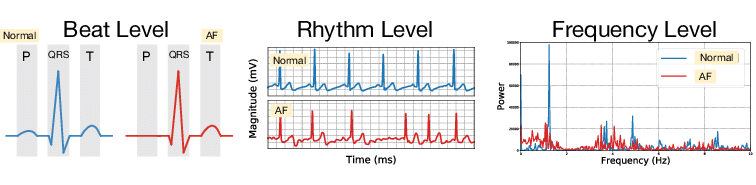
\includegraphics[width=0.9\columnwidth]{media/introduction/NA_ECG_Signal.png}
  \caption{Normal ECG signal (Normal) and Abnormal ECG signal (AF) showing 1. Beat Levels 2. Rhythm Level 3. Frequency Level [\citenum{ref_paper_introduction_1}]}
  \label{fig:normal_abnormal_ecg_signal}
\end{figure}

The detection of arrhythmia from the ECG record is a slow and repetitive process. This process can be shortened by using a machine learning system. Use of machine learning systems will shorten the time required for detection of arrhythmia. This will also reduce the stress from the medical supervisors and staff. As medical facilities have a large number of ECG records, machine learning system will be able to produce extremely accurate results. The use of machine learning will reduce human errors. This will allow the medical professional to focus on more complex problems and better patient care.

In this project, we are using a machine learning system to detect the arrhythmia in COVID-19 patients. The system takes the ECG records from the patients and generates a few models. These models are evaluated and compared against each other. The system employs a weightage-based selection system to select the most-suited model for the task.

\section{Machine Learning}\label{sec:machine_learning_intro_chapter}

Machine learning (ML) is a subset of artificial intelligence (AI) technology. Machine learning is a process in which a computer learns from experience. The machine learning system is used to obtain meaning from the available data. Machine learning uses statistical models and advanced mathematics to find patterns and meaning from provided data. Machine learning does not depend on explicit programming but on learning algorithms derived from various statistical models. The objective of machine learning is to obtain meaningful experience and use this experience to solve complex classification and regression problems. The large amount of data and observations needed to generate a high performance machine learning model Another objective of machine learning is to allow the computer to learn from experience with minimum human interaction.

Machine learning is used in image and speech recognition, recommendation systems, prediction systems, chatbots, classification and detection systems. The use of machine learning is already prominent in the healthcare industry, smart cities, IT industries, R\&D industries, etc. Machine learning takes the data from the users and converts it into structured or unstructured forms. While most algorithms and models prefer structured data, machine learning can utilize both structured and unstructured data according to its needs. For example, machine learning can forecast the amount of solar radiation from various natural elements. Machine learning systems are generally classified into three types:

\subsection{Supervised Learning}\label{subsec:supervised_learning_intro}

The supervised learning systems employ supervised learning algorithms for the learning. This system uses well-labeled data for training. The supervised machine learning algorithm maps the input data against the correct output provided with training data. Supervised algorithms use this learning approach to train themselves for classification and regression tasks.

The performance of supervised learning models is based on the input quality and dimensions of data. The subset of training data is used for the validation process, in which superparameters are trained to increase the performance of models. The supervised learning systems are further categorized into two subsets based on problems.

\subsubsection{Classification Problems}\label{subsubsec:classifcation_problems_intro}

Classification algorithms are a subset of supervised learning algorithms. The classification problems can be binary or multiclass problems. In binary classification, the output is primarily yes or no, true or false. But sometimes classifcation can be different depending on the type of problem. The classification algorithm analyzes the input variables and outputs the class based on the analysis.

\subsubsection{Regression problems}\label{subsubsec:regression_problems_intro}

Regression problems are solved by regressive supervised algorithms. In this problem, algorithms utilize the known relationship between input variables and output variables to train themselves. These algorithms are generally used in the case of forecasting, trend analysis, etc.

\subsection{Unsupervised Learning}\label{subsec:unsupervised_learning_intro}

Unsupervised learning systems are machine learning techniques that employ unsupervised learning algorithms. These algorithms use unlabeled datasets for training purposes. The goal of an unsupervised system is to detect abnormalities in the dataset on its own. This makes the models better suited to unknown environments where they can learn information from any type of data. Unsupervised learning models work better than supervised models in the case of unstructured data as they derive meaning from data without needing human supervision. The advantage of unsupervised learning algorithms is that they are designed to mimic the way of human thinking, making them autonomous and much closer to real artificial intelligence.

There are two major categories of unsupervised learning; they are clustering and assossiation. In the case of clustering, the data points from a dataset are grouped together based on training. These data points are grouped with their similarities to other data points present in the dataset. In the case of association learning systems, the relationship between multiple data points is identified or trends are identified. In other words, association algorithms obtain the relationship between various variables present in a dataset.

\subsection{Reinforcement Learning}\label{subsec:reinforcement_learning_intro}

Reinforcement learning is a subset of supervised learning systems that utilizes feedback based learning systems. In this system, the machine is allowed partial human interaction to analyze its behavior. This system does not use labeled data, but it interacts with the environment on its own. This system is allowed to perform some actions in a given environment and learn from its own experience. This learning system is able to tackle extremely complex and difficult problems due to its dynamic learning approach. But the major disadvantage of this system is its cost-to-performance ratio as well as its longer training time.

Machine learning system is used in this dissertation to detect the arrhyhmia from ECG singals. The system is provided with a template of the five machine learning models, ECG records of the patients, and user preference parameters. The user parameters are used to generate the weightage. The data is split into 80:20 ratios. The system generates the five models using templates and 80\% of the data. These five models are evaluated with weightage and the remaining 20\% of the data.

\section{Problem Statement}\label{sec:problem_statement}
In current COVID-19 pandemic life threatening complications can be avoided with earlier diagnosis. One of such complications is arrhythmia which can be detected by reading ECG signals. This task is carried out by medical personnel. This repetitive and mundane task puts strain on medical staff.

Supervised learning models can be used for such tasks. These models have their own set advantages and disadvantages. Hence automating selection of the best model for required tasks will allow medical personnel to customise applications based on need. This will reduce strain from medical staff and allow them to focus on patient care.

\section{Motivation}\label{sec:motivation}

COVID-19 disease became a global pandemic in 2019. Since then, it has caused around 580 million infections world-wide and 6.42 million deaths, while in India it caused a total of 44.5 million infections, resulting in the deaths of half a million citizens. The infection severity varied from individual to individual, but it has been observed that patients with comorbidities were more likely to result in severe infections. The most common comorbidities observed in these patients were prior respiratory damage caused by other diseases or disorders. The second most common comorbidity was cardiovascular complications.

The cardiovascular comborbidities cause a large number of severe cases and fatalities in COVID-19 patients. The main contributing factor to this was the silent nature of these cardiovascular disorders. Most cardiovascular disorders are hard to detect and left untreated in a large number of cases. Earlier diagnosis of cardiovascular disease will lead to better treatment of patients. This will reduce the number of undetected cases. Cardiovascular diseases are often diagnosed by analyzing ECG records of patients for the presence of arrhythmia. This process is extremely time consuming. Automating this process will reduce the strain placed on medical staff significantly. This will allow them to tackle more complex and important problems. The early diagnosis of cardiovascular disease will allow the proper treatment and patient care for the patient.

During research, we noticed that there was a lack of literature for model selection systems based on user requirements. Therefore, another motivation behind the project is the development of an automated system for the selection of a model. In this system, models are selected from the weightage generated from user choices and performance evaluation of the models. The goal behind the weightage based system is to allow users to give input to the system based on the most important factors. This can be higher accuracy at the cost of prediction time, or lower accuracy at the cost of prediction time. This way, the users are given choice in the selection of the model that will meet their own requirements.

\section{Beneficiaries}\label{sec:beneficiaries}

This system is primarily built for medical personnel tasked with the handling of COVID-19 cases. But it can be beneficial in the cases of patients who suffer from cardiovascular problems and other diseases.

The system is useful for a wide variety of tasks, such as detection of epilepsy or Parkinson's from brain wave charts, and detection of cancer and other disorders. This system will reduce the large amount of workload from the medical staff. The system will help medical personnel get a better understanding of the patients' cases. This will result in better patient treatment and patient care.

Once the system is trained, it can be used for generalized predictions. On the other hand, this system can also be trained for specialized tasks. The system does not need machine learning experts to operate; i.e., it can be trained and used by end users directly. The lack of external connection will also increase security and privacy, while the system will maintain the high performance of the models.

\section{Scope of the project}\label{sec:scope_of_the_project}

Although there are a large number of trained models and systems are present in machine learning, there is a lack of model selection systems targeted towards non-technical people. The aim of this dissertation is to propose an automated model selection system specifically built for non-technical people. This system accepts the user's requirements and provides the most suitable model for their needs.

The system takes a data set in a CSV format file, and the obtained results are returned in JSON format. These JSON files are stored for recording purposes and future use. The dataset provided can be of any dimension, and the data is processed by the pandas library. The dataset used in this process is obtained from the kaggel, and the models are trained with this dataset. The system provides the most suitable model for the prediction depending on the requirements provided by the user and the evaluation of the models.

\section{Organization of Report}\label{sec:organization_of_report}

The report is structure into seven chapters as follows:

\textbf{\textit{Chapter \ref{ch:introduction} - \nameref{ch:introduction}:}}
This chapter gives an overview of the report. It gives a general overview of the current situation of COVID-19 pandemic and the stress it puts on the medical system. It also describes the proposed solution to tackle this problem.

\textbf{\textit{Chapter \ref{ch:literature_survey} - \nameref{ch:literature_survey}:}}
This chapter provides review of relevant literature of supervised learning systems and automation approaches for the model training.

\textbf{\textit{Chapter \ref{ch:system_architecture} - \nameref{ch:system_architecture}:}}
This chapter describes the architecture of the system. It discusses the models used in the system, the automated training and selection of models.

\textbf{\textit{Chapter \ref{ch:system_interface} - \nameref{ch:system_interface}:}}
This chapter describes the user interface of the system. This chapter will discuss the pages accessible by the user and the information about the development server.

\textbf{\textit{Chapter \ref{ch:result_and_analysis} - \nameref{ch:result_and_analysis}:}}
This chapter will describe the performance metrics used by the system for the selection process. The chapter also gives details about the dataset used for training and testing. It also provides recommended system specification required by the application.

\textbf{\textit{Chapter \ref{ch:applications} - \nameref{ch:applications}:}}
This chapter gives various applications of the developed system.

\textbf{\textit{Chapter \ref{ch:conclusion_and_future_scope} - \nameref{ch:conclusion_and_future_scope}:}}
This chapter concludes the report by providing a brief summary of the project. This chapter also describes the future scope of the system.
